\section{FAT}
\subsection{Introducción}
\begin{frame}{Introducción}
  \begin{itemize}
    \item Creado por Bill Gates y Marc McDonald.
    \item Se creó en 1977.
    \item Su primera versión fue FAT12 (con direcciones de 12 bits).
    \item Posteriormente apareció FAT16.
    \item Finalmente se llegó a FAT32 (el actual) (28 bits).
  \end{itemize}
\end{frame}

\subsection{Características}
\begin{frame}{Características}
  \begin{itemize}
    \item Tamaño máximo: 32GB
    \item Tamaño máximo de fichero: 4GB
    \item Máximo de caracteres de nombre de fichero: 255B
    \item Máximo número de ficheros: 4.177.920
  \end{itemize}
\end{frame}

\subsection{Estructura}
\begin{frame}{Estructura}
  \begin{itemize}
    \item Al principio de la partición nos encontramos el sector de arranque.
    \item Justo después se encuentra la FAT
    \item Normalmente (pero no necesariamente) encontramos después el directorio raíz.
    \item Después nos encontramos el área de datos, donde se almacenan todos los ficheros.
  \end{itemize}
\end{frame}

\begin{frame}{Estructura}
  \begin{center}
    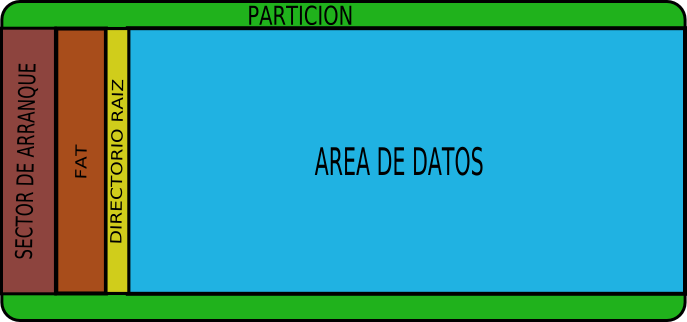
\includegraphics[height=5.5cm]{imgs/fat_struct.png}
  \end{center}
\end{frame}

\begin{frame}{Ficheros}
  \begin{itemize}
    \item Los ficheros única y exclusivamente contienen datos y están almacenados en el sector de datos de la partición.
    \item Las entradas de directorios almacenan el nombre, el número de cluster y los atributos de cada uno de los ficheros que contiene.
    \item Los ficheros vacíos no contienen ocupan bloques de datos ni entradas en la fat.
    \item Si un cluster no es el ultimo del fichero, contiene el número de cluster siguiente, si lo es, contiene una marca.
    \item Los directorios siempre contiene como mínimo los subdirectorios \".\" y \"..\", excepto el directorio raíz.
  \end{itemize}
\end{frame}

\begin{frame}{Ficheros}
  \begin{center}
    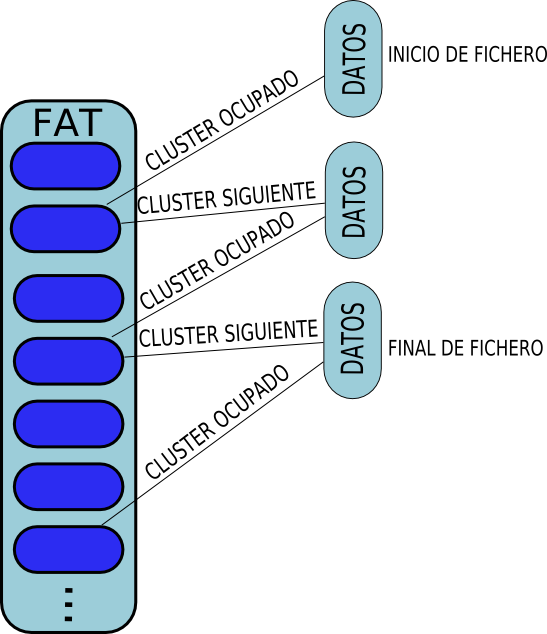
\includegraphics[height=6cm]{imgs/fat_files.png}
  \end{center}
\end{frame}
